\input{../include/preamble}

\title[ID1019 Overview]{Overview}


\author{Johan Montelius}
\institute{KTH}
\date{\semester}

\begin{document}

\begin{frame}
\titlepage
\end{frame}


\begin{frame}{Introduction}
  \begin{itemize}
    \pause \item Registration
    \pause \item Learning outcomes
    \pause \item Literature
    \pause \item Lectures
    \pause \item Seminars
    \pause \item Exam
    \pause \item More
  \end{itemize}
\end{frame}

\begin{frame}{Registration}
  Register in KTH-Social - if there is a problem:
\pause
  \begin{itemize}
    \item you have not done course selection,
    \item you have not done registration for the semester (``terminsregistrering'') or
    \item you do not fullfill the course prerequisite
  \end{itemize}
\pause
  Make sure to registered for the course.
\end{frame}

\begin{frame}{Learning outcomes}
  The aim of the course:

\pause
\begin{itemize}
\item Functional programming:
\pause
  \begin{itemize}
   \item recursion, pattern matching, functions as first class objects, closures, higher order functions and in-mutable data structures
\pause
   \item implement selected algorithms in a functional programming language
  \end{itemize}
\pause
\item Concurrent programming:
  \begin{itemize}
\pause
    \item advantages and disadvantages
\pause
    \item shared memory, message passing
\pause
    \item design, implement, test and debug 
  \end{itemize}  
\end{itemize}

\end{frame}


\begin{frame}{why functional programming}

Why do we need a course in functional and concurrent programming?

\begin{tikzpicture}[scale=1.0]
\pause
 \node (haskell) at (1,6) {
\includegraphics[scale=0.4]{haskell.png}};
\pause
 \node (lisp) at (6,7) {
\includegraphics[scale=0.3]{lisp.png}};
\pause
 \node (erlang) at (0,2) {
\includegraphics[scale=0.6]{erlang.jpeg}};
 \pause
 \node (f) at (10,6) {
\includegraphics[scale=0.4]{f.jpeg}};
\pause 
 \node (scala) at (4,4) {
\includegraphics[scale=0.1]{scala.png}};
\pause
 \node (python) at (4,2) {
\includegraphics[scale=0.4]{python.png}};
\pause
 \node (c11) at (10,2) {
\includegraphics[scale=0.3]{c11.jpeg}};
\end{tikzpicture}

\end{frame}

\begin{frame}{why concurrency}

Two reasons:

\pause\vspace{20pt}\hspace{60pt}A tool to model interactive services.

\pause\vspace{20pt}\hspace{60pt}Hardware can utilize concurrency to speed-up computations.

\pause\vspace{40pt}
{\em To build a good game engine, you need to master concurrency}

\end{frame}


\begin{frame}{Literature}

\pause
\begin{columns}
 \begin{column}{0.6\linewidth}
  \begin{itemize}
    \item ``Erlang Programming'', Cesarini and Thompson, O'Reilly 2009
    \item ``Programming Erlang'', Joe Armstrong
    \item ``Erlang and OTP in Action'', Martin Logan, Eric Merritt, and Richard Carlsson
  \end{itemize}
 \end{column}
 \begin{column}{0.4\linewidth}
  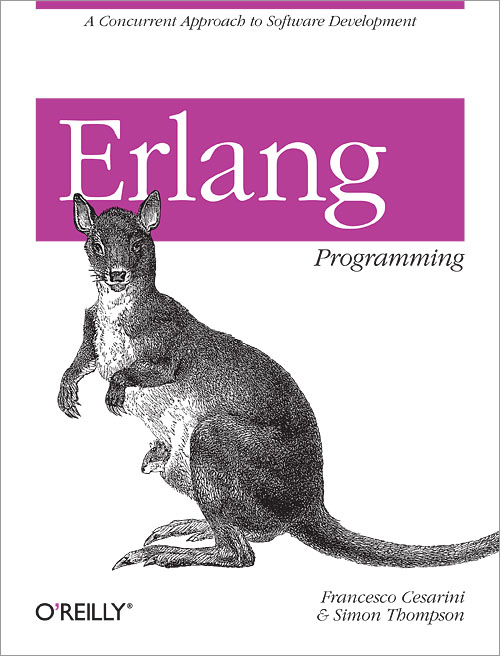
\includegraphics[width=\linewidth]{coursebook.jpg}
 \end{column}
\end{columns}
  
\end{frame}


\begin{frame}{Online content}

   Collaboration with Erlang Solutions (not confirmed):

\begin{columns}
 \begin{column}{0.6\linewidth}
  \begin{itemize}
       \item online video lectures
       \item quizzes and assignments 
       \item follows the book
  \end{itemize}
 \end{column}
 \begin{column}{0.4\linewidth}
  
\includegraphics[width=\linewidth]{logo.png}
 \end{column}
\end{columns}

\vspace{20pt}
{\em The main source for learning Erlang is the course book and the
video tutorials. You will not learn Erlang just by following the
lectures!}

\end{frame}


\begin{frame}{Lectures}

   We will have 14 lectures that will complement the course literature
   and introduce topics that are not covered by the book.

  \begin{itemize}
    \item Functional programming
\pause
    \item Programming techniques
\pause
    \item Complexity 
\pause
    \item Concurrency 
\pause
    \item Parallelism
\pause
    \item Servers
  \end{itemize}
\end{frame}


\begin{frame}{Seminars}

  To take part in the seminar sessions, you should:
  \begin{itemize}
  \item solve an assigment before the seminar
  \end{itemize}

  \pause \vspace{20pt}
  The seminars are not compulsory but,\pause if you attend you should have prepared well. 

  \pause \vspace{20pt}
  Collaborate in the implementation.

\end{frame}

\begin{frame}{Seminars}
  \begin{itemize}
    \item Huffman coding: implementing a compression algorithm \pause
    \item A meta-interpreter: Erlang interpreter in Erlang \pause
    \item Dining philosophers: introduction to concurrency \pause
    \item A Mandelbrot image: parallelism \pause
    \item A small web server: easier than you think
  \end{itemize}
\end{frame}

\begin{frame}{Exam}

\pause A closed book exam -- {\bf where writing code by hand will be a large part.}

\vspace{20pt}

\pause Final grade is based on written exam. 

\end{frame}

\begin{frame}{and finally}

  Two student representatives for course board. We will meet a couple
  of times during the course so that you can give feedback.

\pause\vspace{20pt}

Don't use KTH Social for feedback or questions, email me
johanmon@kth.se, or talk to your student representatives.

\end{frame}

\end{document}
